\section{A expansão comercial}

A espaçonave \emph{Dragon 1}, da \emph{SpaceX}, desempenha um papel importante no transporte de cargas e na devolução de experimentos científicos da ISS para a Terra, tornando-a indispensável para a realização de estudos científicos avançados em ambientes de microgravidade.
Como exemplificado por \cite{bell2018}, a \emph{Dragon} trouxe uma carga de dados científicos que incluem pesquisas em biologia, estudo realizado por \cite{chamberlain2021} na área da ciência dos materiais e fisiologia humana, como escrito por \cite{wang2018}.
Esses resultados ajudam a avançar na compreensão dos desafios de missões espaciais de longa duração, como aquelas planejadas para a Lua e Marte \cite{nasaDragonReturn}.

Além disso, a \emph{Dragon 1} demonstrou avanços em tecnologias de reentrada e aterrissagem seguras e de forma que possam reutilizar o mesmo equipamento para missões futuras \cite{nasaFalcon9Dragon}.
Após se desacoplar da ISS, a espaçonave reentrou na atmosfera terrestre e pousou em uma plataforma drone retangular no Oceano Pacífico, como descrito por \cite{nasaspaceflightDroneShip}.

\subsection{Atracação da espaçonave Dragon 1}

A espaçonave \emph{Dragon 1} utiliza tecnologias avançadas de \emph{Light Detection and Ranging} (LiDAR) e de navegação por posicionamento global (GPS) para realizar manobras autônomas até a ISS, como explicado por \cite{nasaspaceflightDragonISS}.
O LiDAR fornece medições tridimensionais da distância e da orientação da espaçonave em relação à ISS, permitindo que a \emph{Dragon 1} ajuste continuamente sua atitude durante as fases de aproximação; e de forma simultânea, o sistema GPS integrado oferece dados de localização em tempo real.

Essas tecnologias em conjunto permitem que a \emph{Dragon 1} alcance o ponto de captura designado com mínima intervenção humana.
Uma vez em posição, o braço robótico \emph{Canadarm2}, operado pelos astronautas a bordo da ISS, é utilizado para capturar e conectar a Dragon ao porto de acoplamento.

\begin{figure}[H]
    \centering
    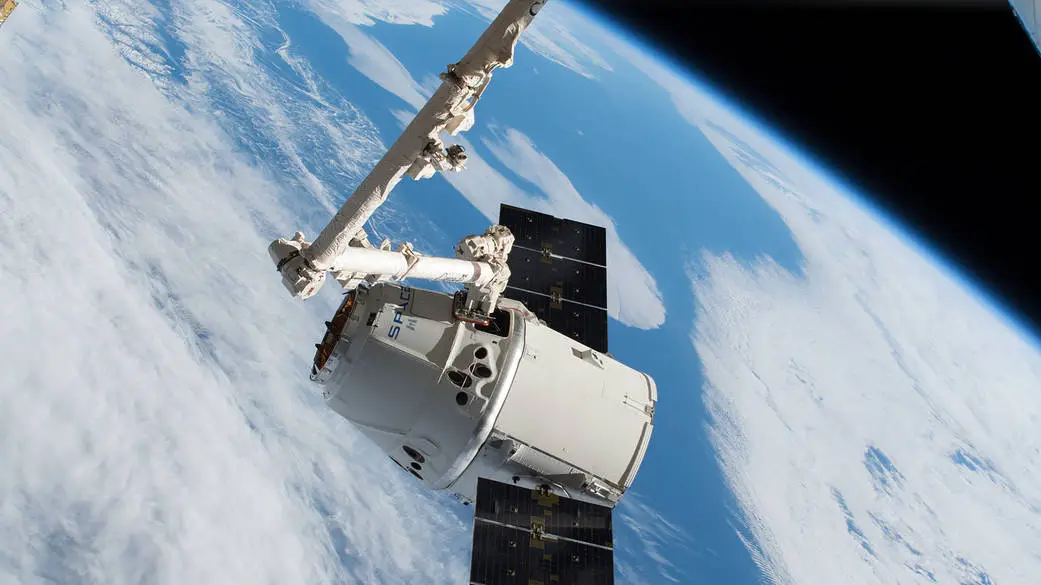
\includegraphics[width=1\linewidth]{1 Introducao/Imagens/SpaceXDragonCanadarm2Foto1.png}
    \caption{Espaçonave Dragon sendo capturada pelo Canadarm2. Fonte: NASA.}
    \label{fig_DragonCadanarm2Foto}
\end{figure}